\chapter{Numerical experiments}
\label{ch:experiments}

Chapter~\ref{ch:motivation} showed that the $2^{B}$ mask space is diverse and that the all-target mask is not in the top cluster. This chapter reports the core result: REINFORCE on 14 Bernoulli logits finds good masks on FLUX.2 within a few hundred image evaluations and beats the all-ones baseline on every task.

\section{Setup}
\label{sec:experiments_seg}

The generator is the FLUX.2-klein-base-9B rectified-flow model (Section~\ref{sec:methods_reinforce}). The source image comes from running the source prompt through FLUX with a fixed noise seed; every candidate mask reuses the same noise, so only the conditioning schedule varies between runs. No inversion step enters the pipeline. All 15 background-rich edits use $N=14$ bits, $T=28$ denoising steps ($R=2$), $512{\times}512$ resolution, and CFG scale $4.0$. SAM~3.1 produces the foreground mask (fallback: Grounding-DINO+SAM~2, then CLIPSeg). The reward follows Equation~\ref{eq::reward_reinforce} with $\alpha=0.7$; the vision-language backbone for $f_{\text{fg}}$ is \texttt{google/siglip2-so400m-patch14-384}.

\section{REINFORCE on 15 background-rich tasks}
\label{sec:experiments_new_bgrich}

\subsection{Task suite}

The 15 edit pairs put a small object inside a rich scene. Example source prompt: ``antique terrestrial globe on a polished dark mahogany desk in a Victorian study, surrounded by stacks of leather-bound books, a brass compass, \dots'' The target prompt changes only the object token: ``brass mechanical orrery on a polished dark mahogany desk\dots'' A rich background gives $f_{\text{bg-ssim}}$ room to drop when the mask over-edits, so the reward can tell a good mask from a lazy one. The 15 pairs are: camera$\to$binoculars, chess$\to$checkers, crown$\to$tiara, globe$\to$orrery, guitar$\to$banjo, lantern$\to$candelabra, piano$\to$harp, pocketwatch$\to$compass, revolver$\to$flintlock, sewing$\to$typewriter, skull$\to$hourglass, teapot$\to$samovar, telescope$\to$microscope, violin$\to$cello, wine$\to$whiskey.

Each run uses 80 episodes $\times$ 8 masks per batch $=$ 640 generations, about $25\times$ cheaper than the $2^{14}=16{,}384$ exhaustive budget.

\subsection{Main result: learning curves}

Figure~\ref{fig::new_bgrich_curves} is the central empirical result of the thesis. Each thin coloured line is one edit; the thick black line is the mean $\pm$ std across the 15 tasks. The dotted red line shows the all-ones reward averaged to $0.601$.

\begin{figure}[H]
    \centering
    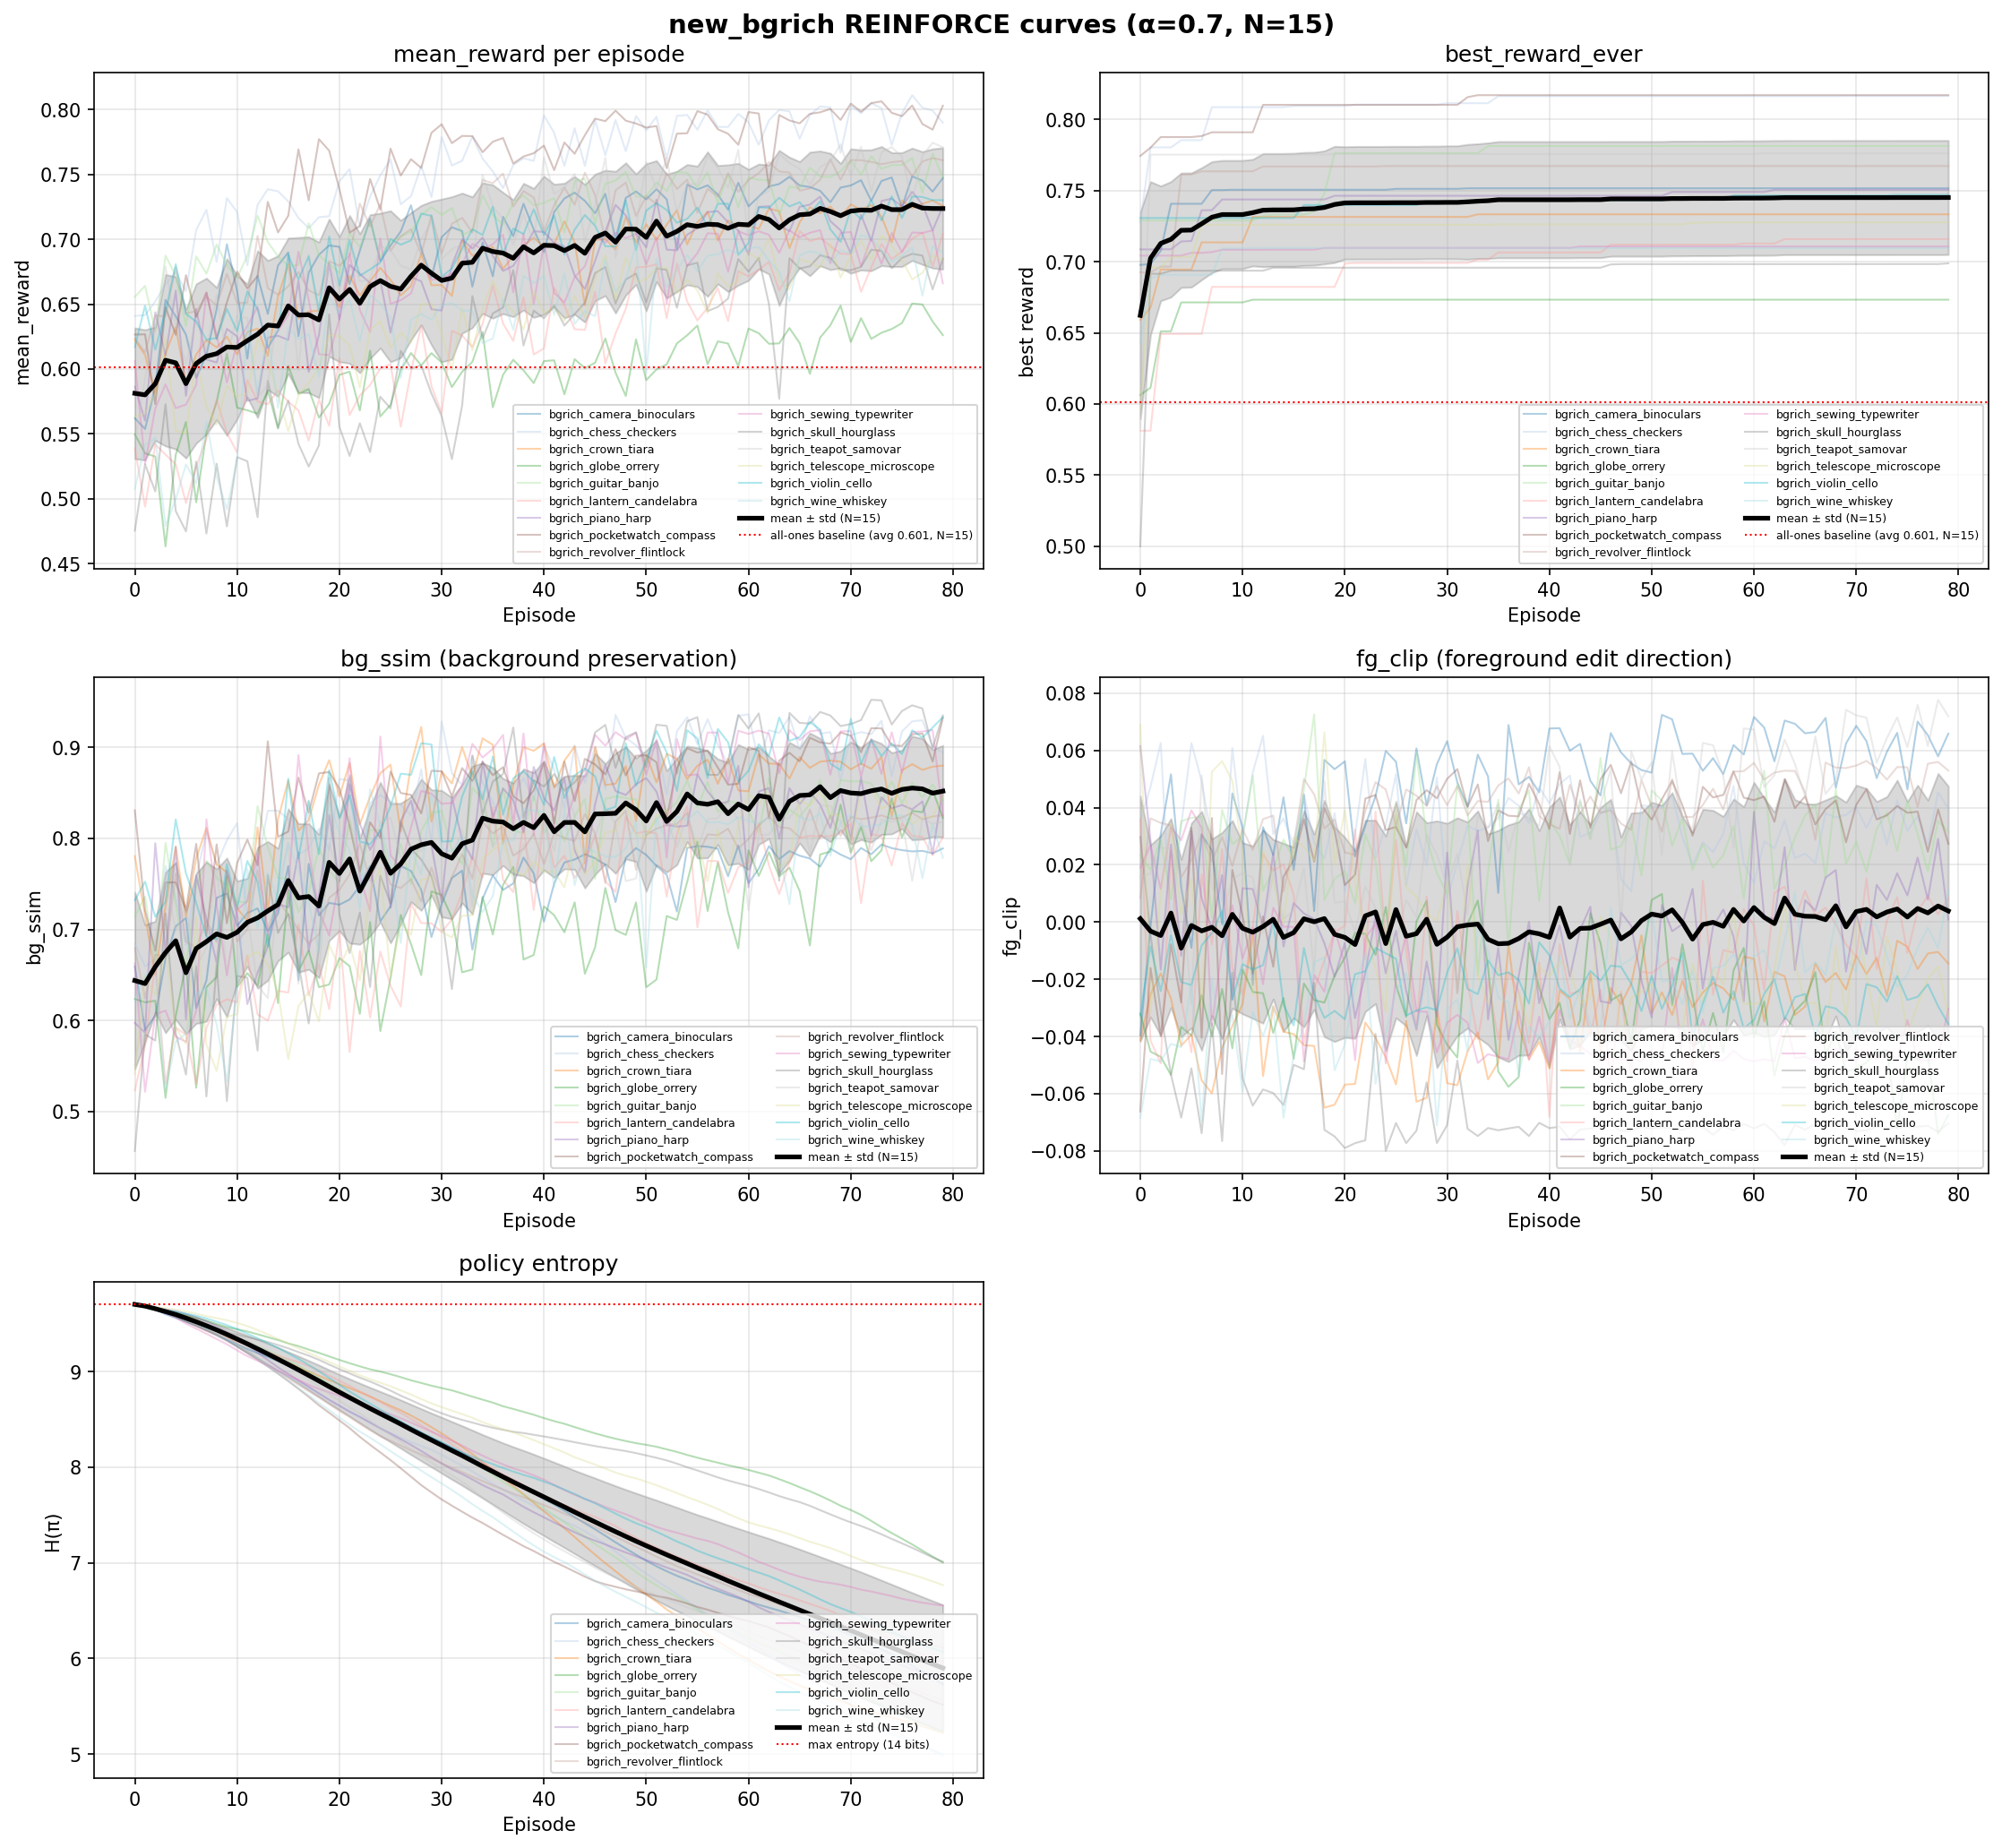
\includegraphics[width=\textwidth]{images/phase2/new_bgrich_training_curves.png}
    \caption{REINFORCE training curves on 15 background-rich editing tasks (FLUX.2, $\alpha=0.7$, $N=14$, 80 episodes $\times$ 8 masks). Top-left: mean batch reward per episode. The policy crosses the all-ones baseline (red dashed, $0.601$) inside the first ten episodes and plateaus near $0.73$. Top-right: best reward ever. About 80\% of the final best is already in hand by episode~10. Middle row: background SSIM climbs from $0.65$ to $0.85$; mean foreground CLIP (the delta-direction cosine) hovers near zero. Bottom: policy entropy drops from $9.7$ (maximum for 14 bits) to ${\sim}6.5$; the policy sharpens but does not collapse.}
    \label{fig::new_bgrich_curves}
\end{figure}

Four observations follow from Figure~\ref{fig::new_bgrich_curves}.

\paragraph{(1) REINFORCE beats the all-ones baseline on all 15 tasks.} The mean best-reward-ever line rises above the all-ones line inside the first ten episodes and stays above it for every individual edit, including the weakest starts (wine$\to$whiskey and skull$\to$hourglass). The mean margin over all-ones is $+0.148$ reward ($+23\%$ relative).

\paragraph{(2) Most of the improvement happens in the first 80 generations.} Best-reward-ever is within $5\%$ of its final value by episode~10 ($=\!80$ generations). The remaining 70 episodes sharpen the policy without much extra reward. This short ramp explains the $25\times$ cost reduction relative to exhaustive $2^{14}$ search.

\paragraph{(3) The gain comes from background preservation, not foreground.} The $f_{\text{bg-ssim}}$ curve improves monotonically from $0.65$ to $0.85$. The $f_{\text{fg-clip}}$ curve stays flat near zero. Under $\alpha=0.7$ on a background-rich scene, the all-ones trajectory already hits a decent foreground match, and the policy's job is to stop the background from collapsing.

\paragraph{(4) The policy sharpens but does not collapse.} Entropy drops from $14\log 2 \approx 9.7$ to $\sim 6.5$, about two bits per timestep on average. The policy commits hard on some bits and stays soft on others. The dual early-stop rule (plateau on mean-reward, or $H<0.5$) keeps the entropy above the collapse threshold.

\subsection{Per-task numbers}

Table~\ref{tab::new_bgrich_numbers} lists per-task all-ones reward, REINFORCE final best-reward, and the gap.

\begin{table}[H]
    \centering
    \caption{All-ones baseline vs.\ REINFORCE best-of-640 on 15 background-rich tasks (FLUX.2, $\alpha=0.7$).}
    \begin{tabular}{lccc}
    \toprule
    Task & All-ones $R$ & REINFORCE best $R$ & $\Delta$ \\
    \midrule
    camera$\to$binoculars       & 0.612 & 0.751 & +0.140 \\
    chess$\to$checkers          & 0.686 & 0.783 & +0.097 \\
    crown$\to$tiara             & 0.589 & 0.733 & +0.144 \\
    globe$\to$orrery            & 0.561 & 0.676 & +0.115 \\
    guitar$\to$banjo            & 0.695 & 0.820 & +0.125 \\
    lantern$\to$candelabra      & 0.569 & 0.730 & +0.161 \\
    piano$\to$harp              & 0.611 & 0.743 & +0.133 \\
    pocketwatch$\to$compass     & 0.602 & 0.773 & +0.171 \\
    revolver$\to$flintlock      & 0.622 & 0.782 & +0.160 \\
    sewing$\to$typewriter       & 0.538 & 0.744 & +0.206 \\
    skull$\to$hourglass         & 0.547 & 0.740 & +0.193 \\
    teapot$\to$samovar          & 0.604 & 0.743 & +0.140 \\
    telescope$\to$microscope    & 0.636 & 0.787 & +0.150 \\
    violin$\to$cello            & 0.668 & 0.778 & +0.110 \\
    wine$\to$whiskey            & 0.478 & 0.654 & +0.176 \\
    \midrule
    \textbf{mean}               & \textbf{0.601} & \textbf{0.749} & \textbf{+0.148} \\
    \bottomrule
    \end{tabular}
    \label{tab::new_bgrich_numbers}
\end{table}

Every task improves. The smallest gain, $+0.097$ on chess$\to$checkers, still exceeds the between-task standard deviation of the all-ones baseline. Tasks with the lowest all-ones reward (wine$\to$whiskey, sewing$\to$typewriter) gain the most in absolute terms: the policy puts its capacity where the all-ones trajectory is most broken.

\section{Single-edit hyperparameter sweep}
\label{sec:experiments_sweep}

Before running the 15-edit suite we swept 8 hyperparameter configurations in parallel on 8 GPUs for one edit at a time. Configurations varied $\alpha\in\{0.3, 0.5, 0.7\}$, the learning rate, and the entropy coefficient. Each configuration ran a fixed 80-episode budget (640 generations) with no early stop, for a direct comparison. Figures~\ref{fig::sweep_typewriter}--\ref{fig::sweep_penguin} show three representative sweeps.

\begin{figure}[H]
    \centering
    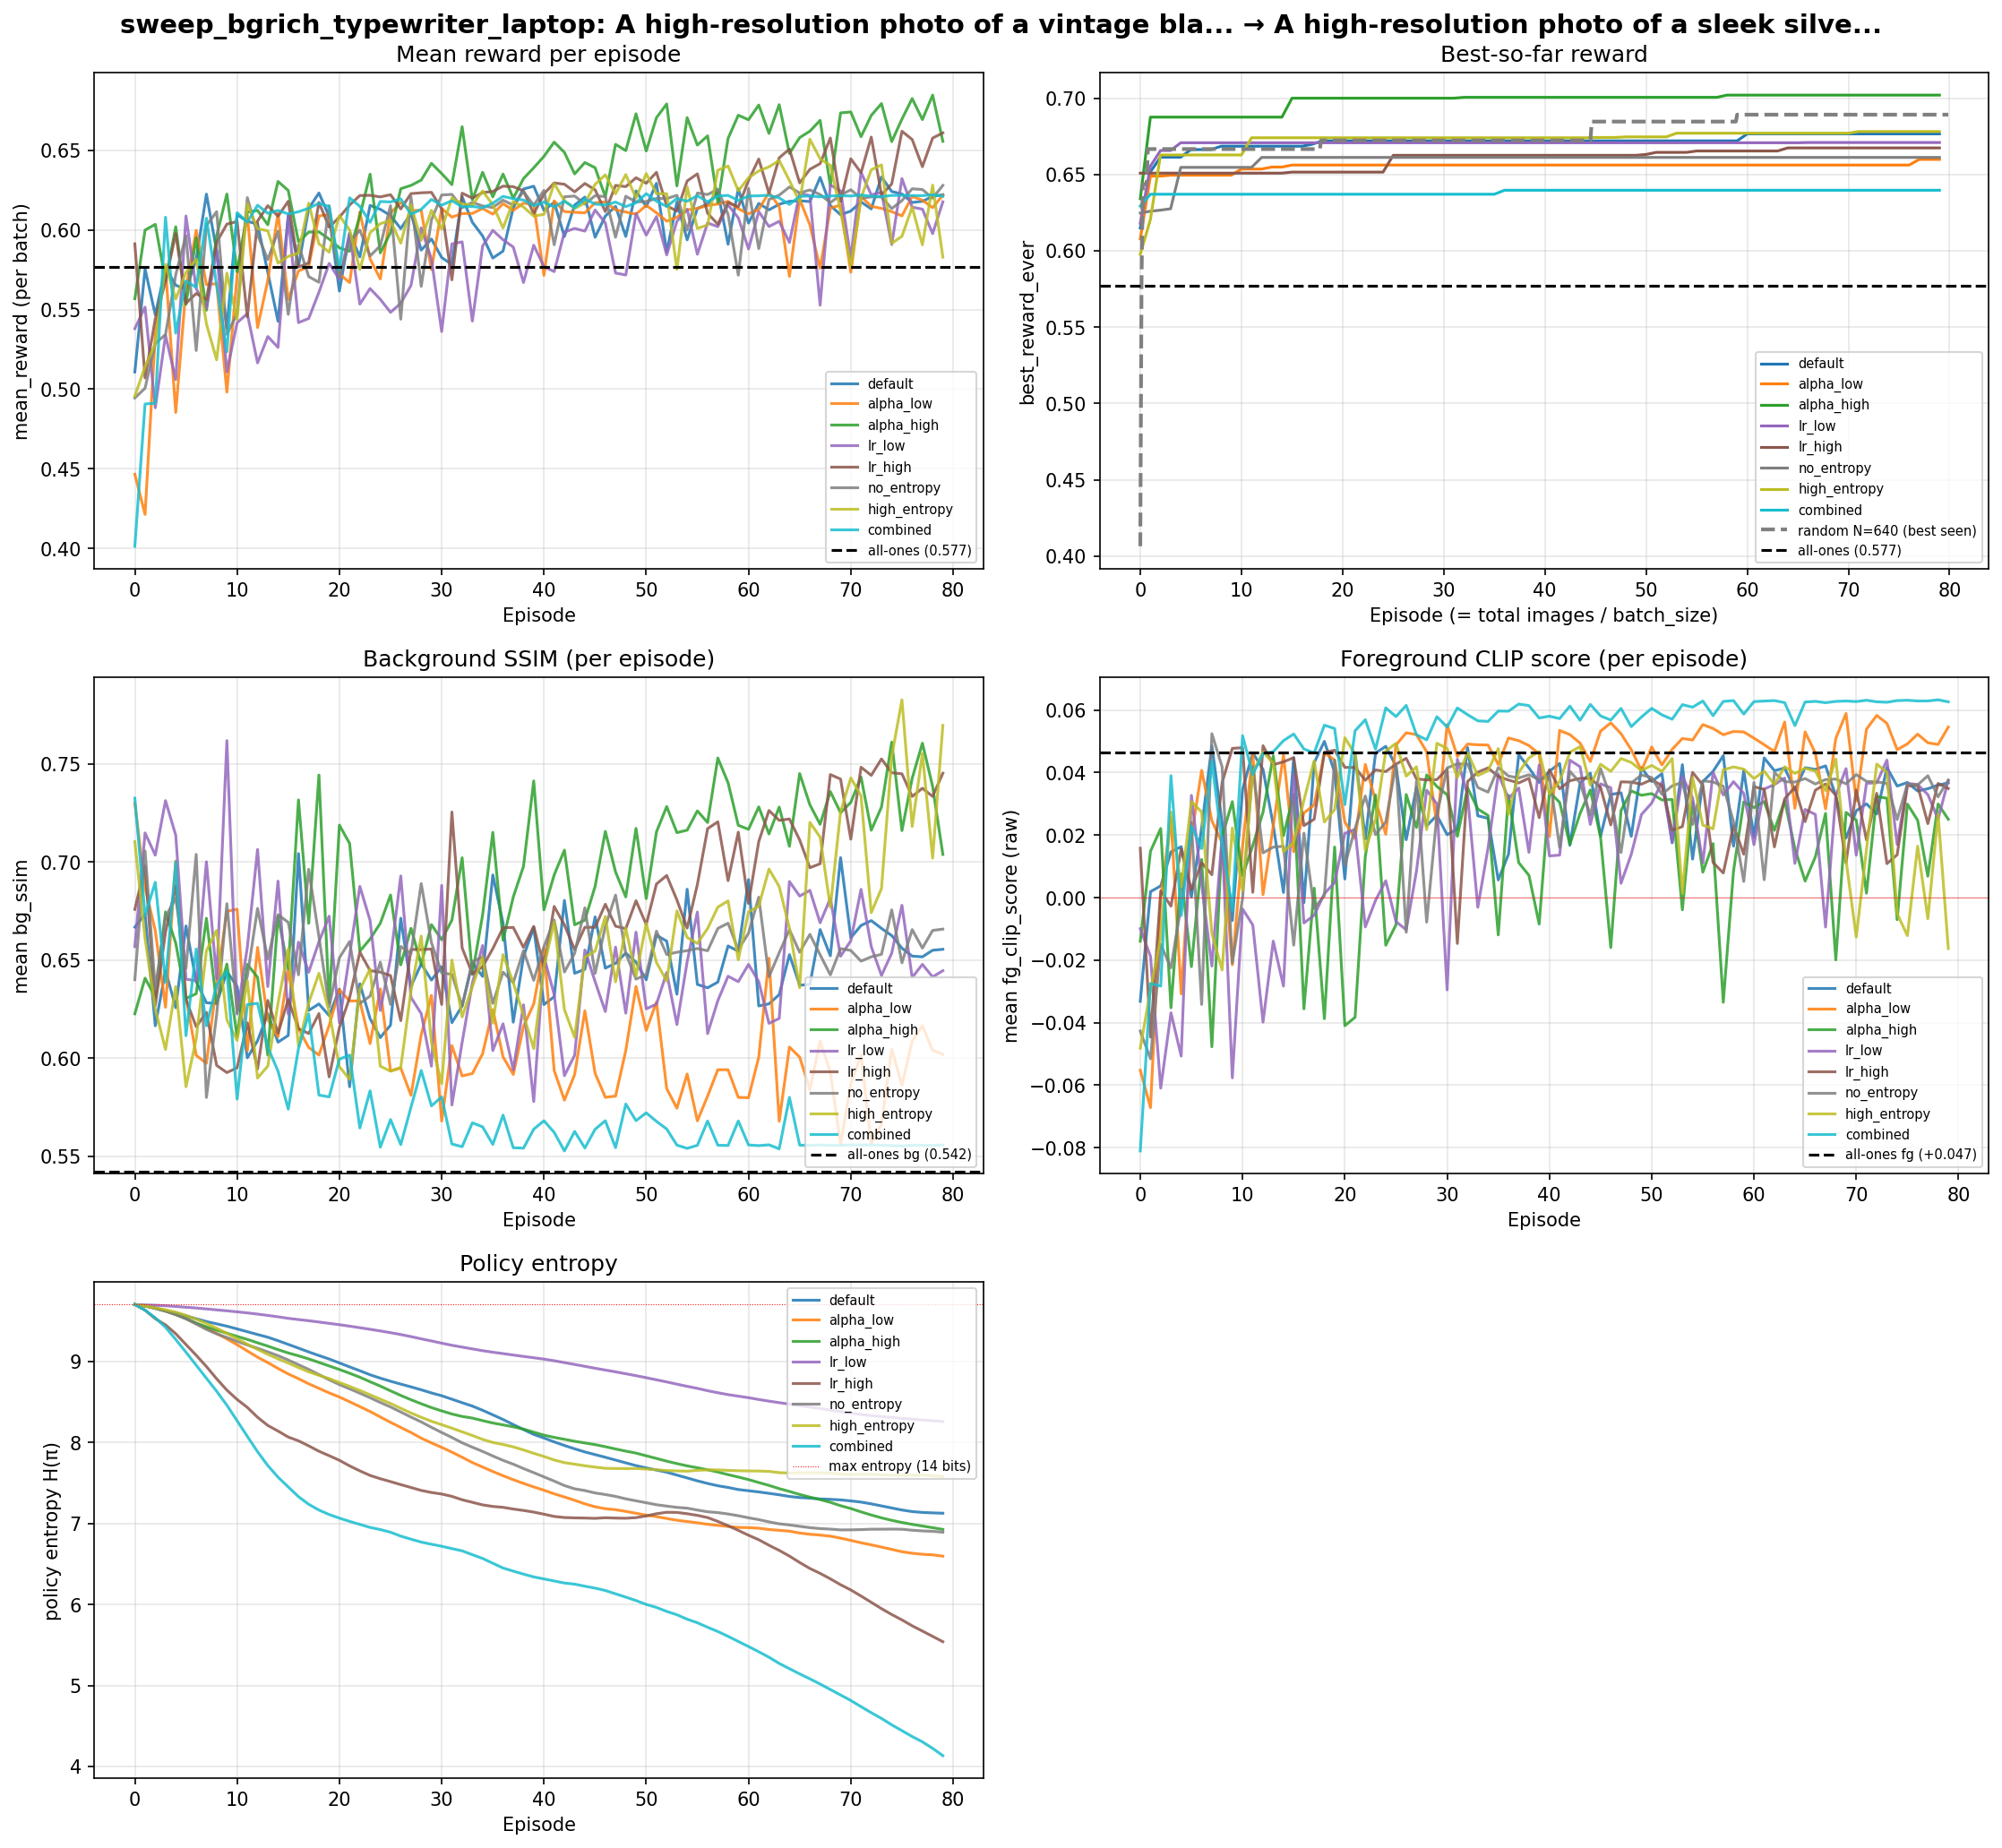
\includegraphics[width=\textwidth]{images/phase2/sweep_typewriter_laptop_curves.png}
    \caption{8-config sweep on \texttt{bgrich\_typewriter\_laptop}. All-ones reward $0.577$. Best config \texttt{alpha\_high} reaches $0.702$; random-640 best $0.689$. Every REINFORCE config matches or beats random at matched budget.}
    \label{fig::sweep_typewriter}
\end{figure}

\begin{figure}[H]
    \centering
    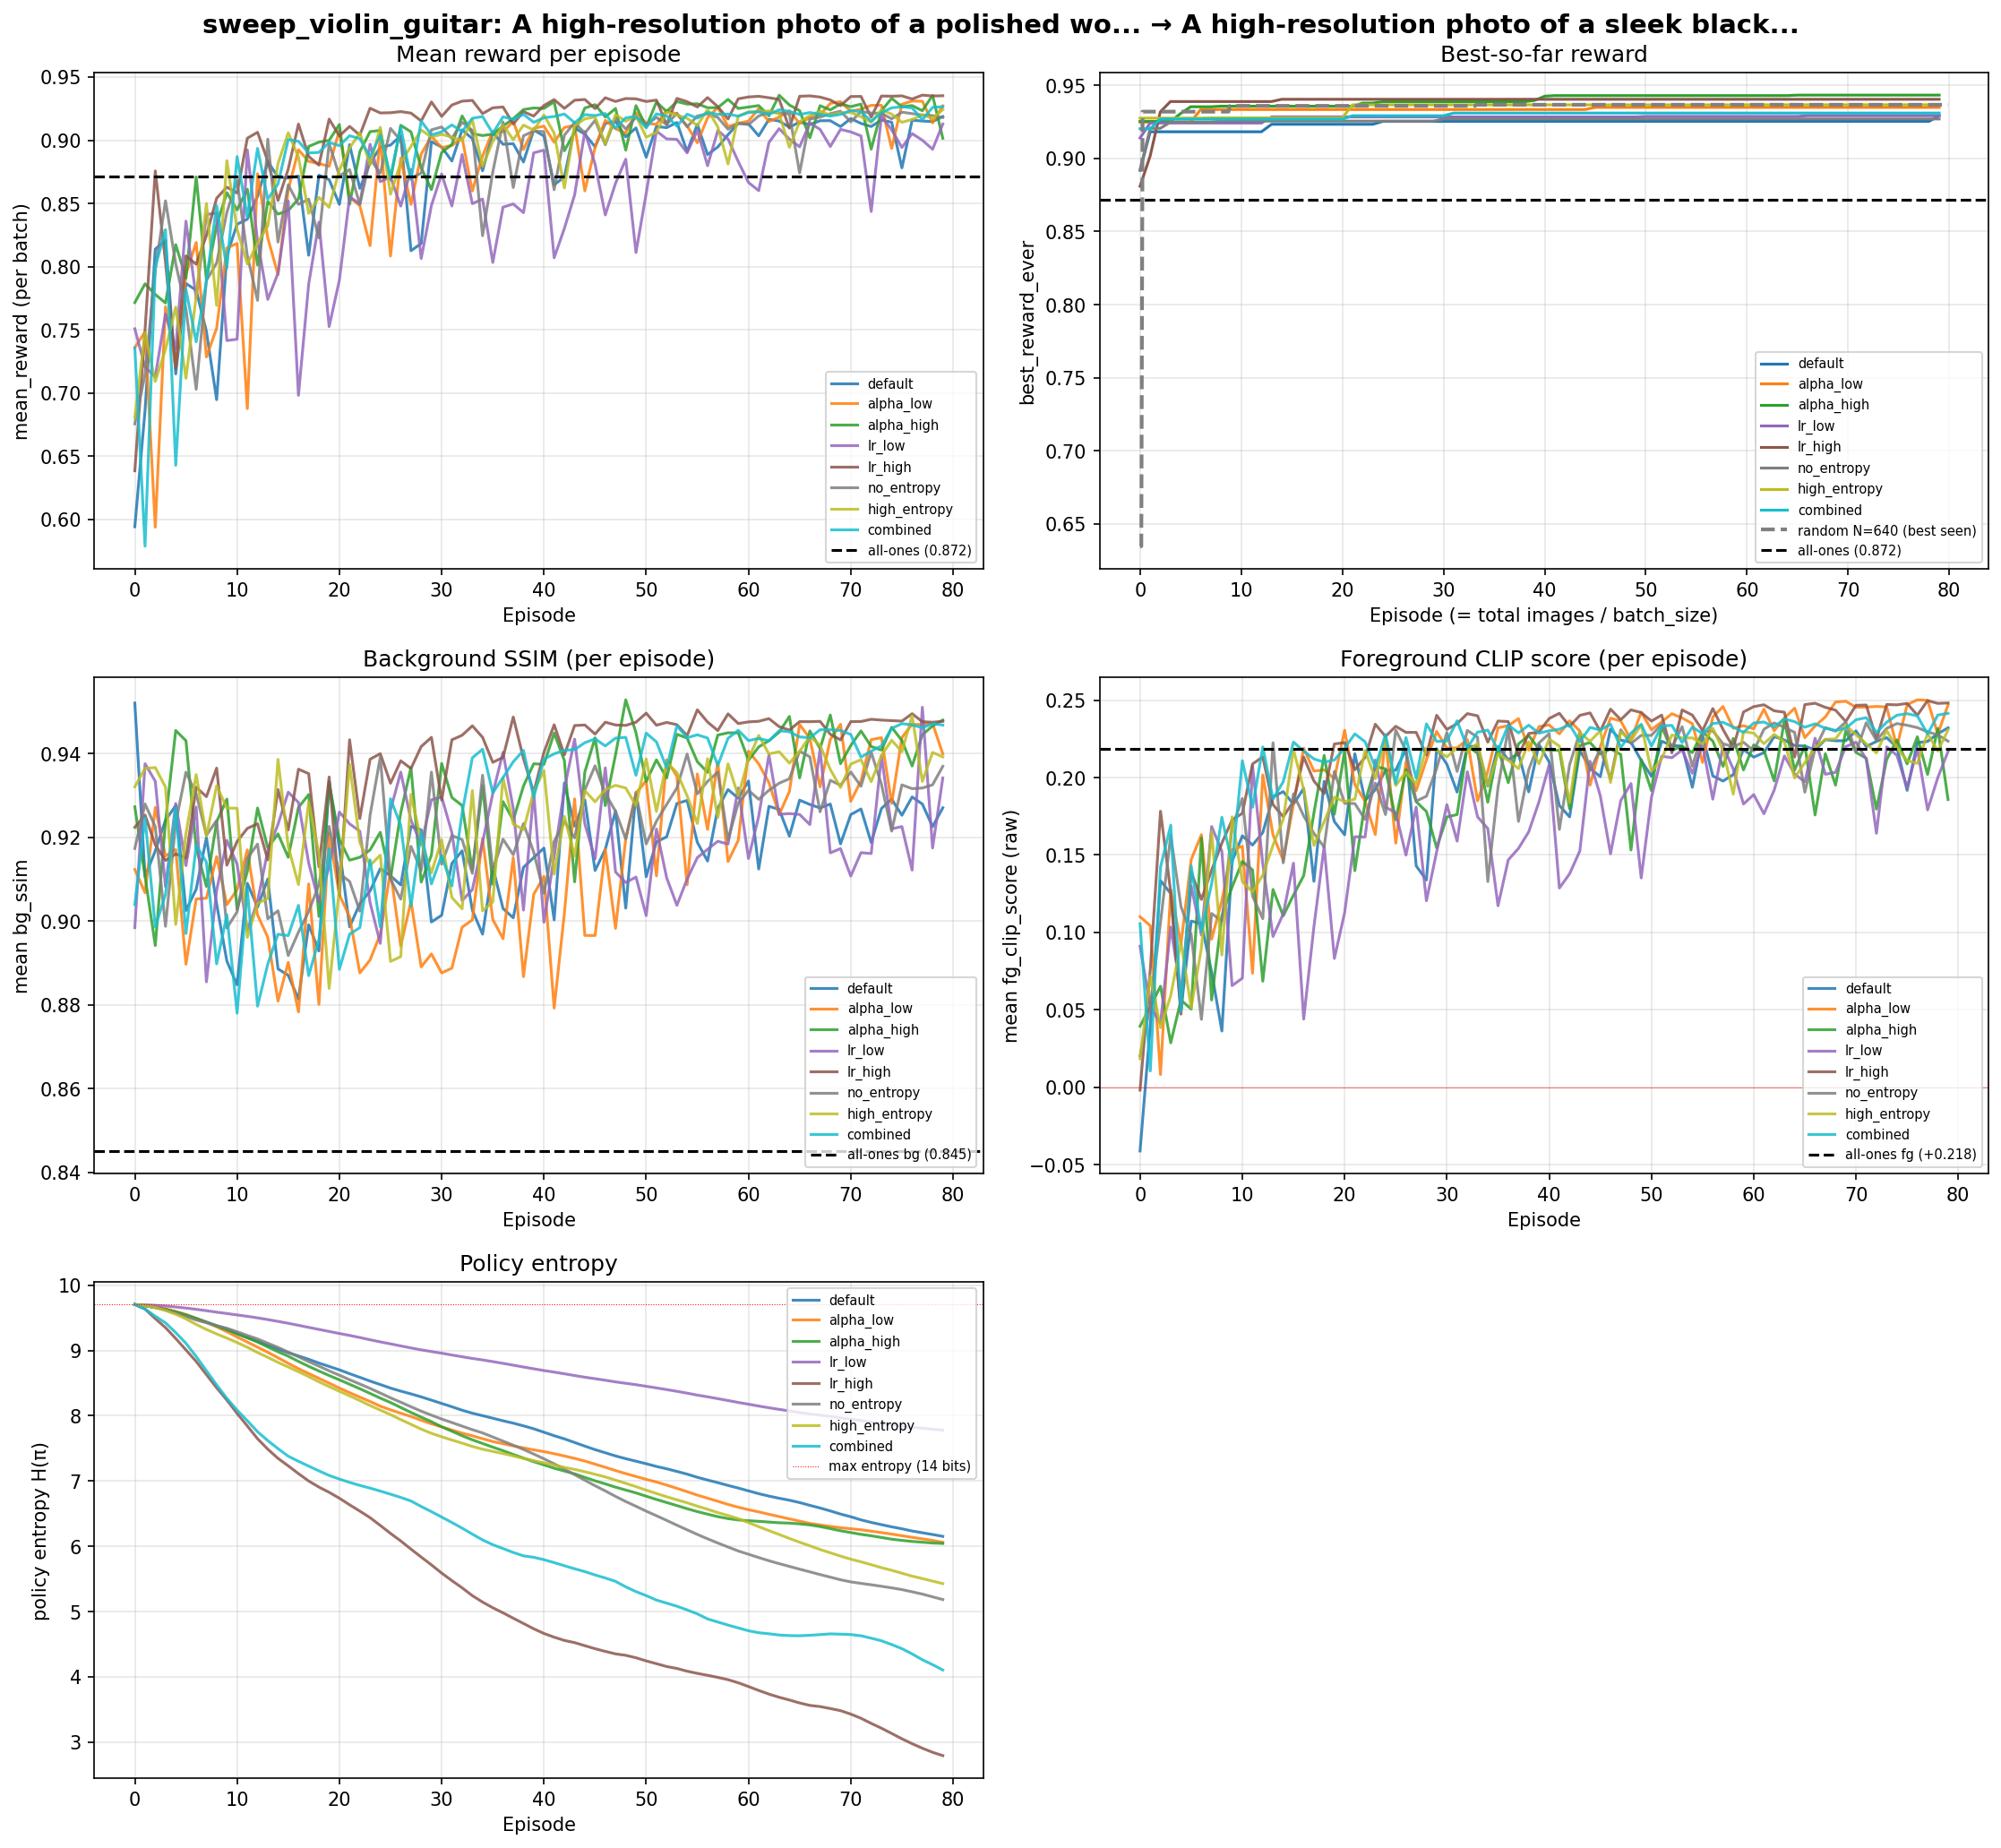
\includegraphics[width=\textwidth]{images/phase2/sweep_violin_guitar_curves.png}
    \caption{8-config sweep on \texttt{violin\_guitar}. All-ones reward $0.872$ (violin already scores well against ``guitar''). Best config \texttt{alpha\_high} reaches $0.943$; random-640 best $0.937$. Smaller absolute headroom; REINFORCE still finds a better mask.}
    \label{fig::sweep_violin}
\end{figure}

\begin{figure}[H]
    \centering
    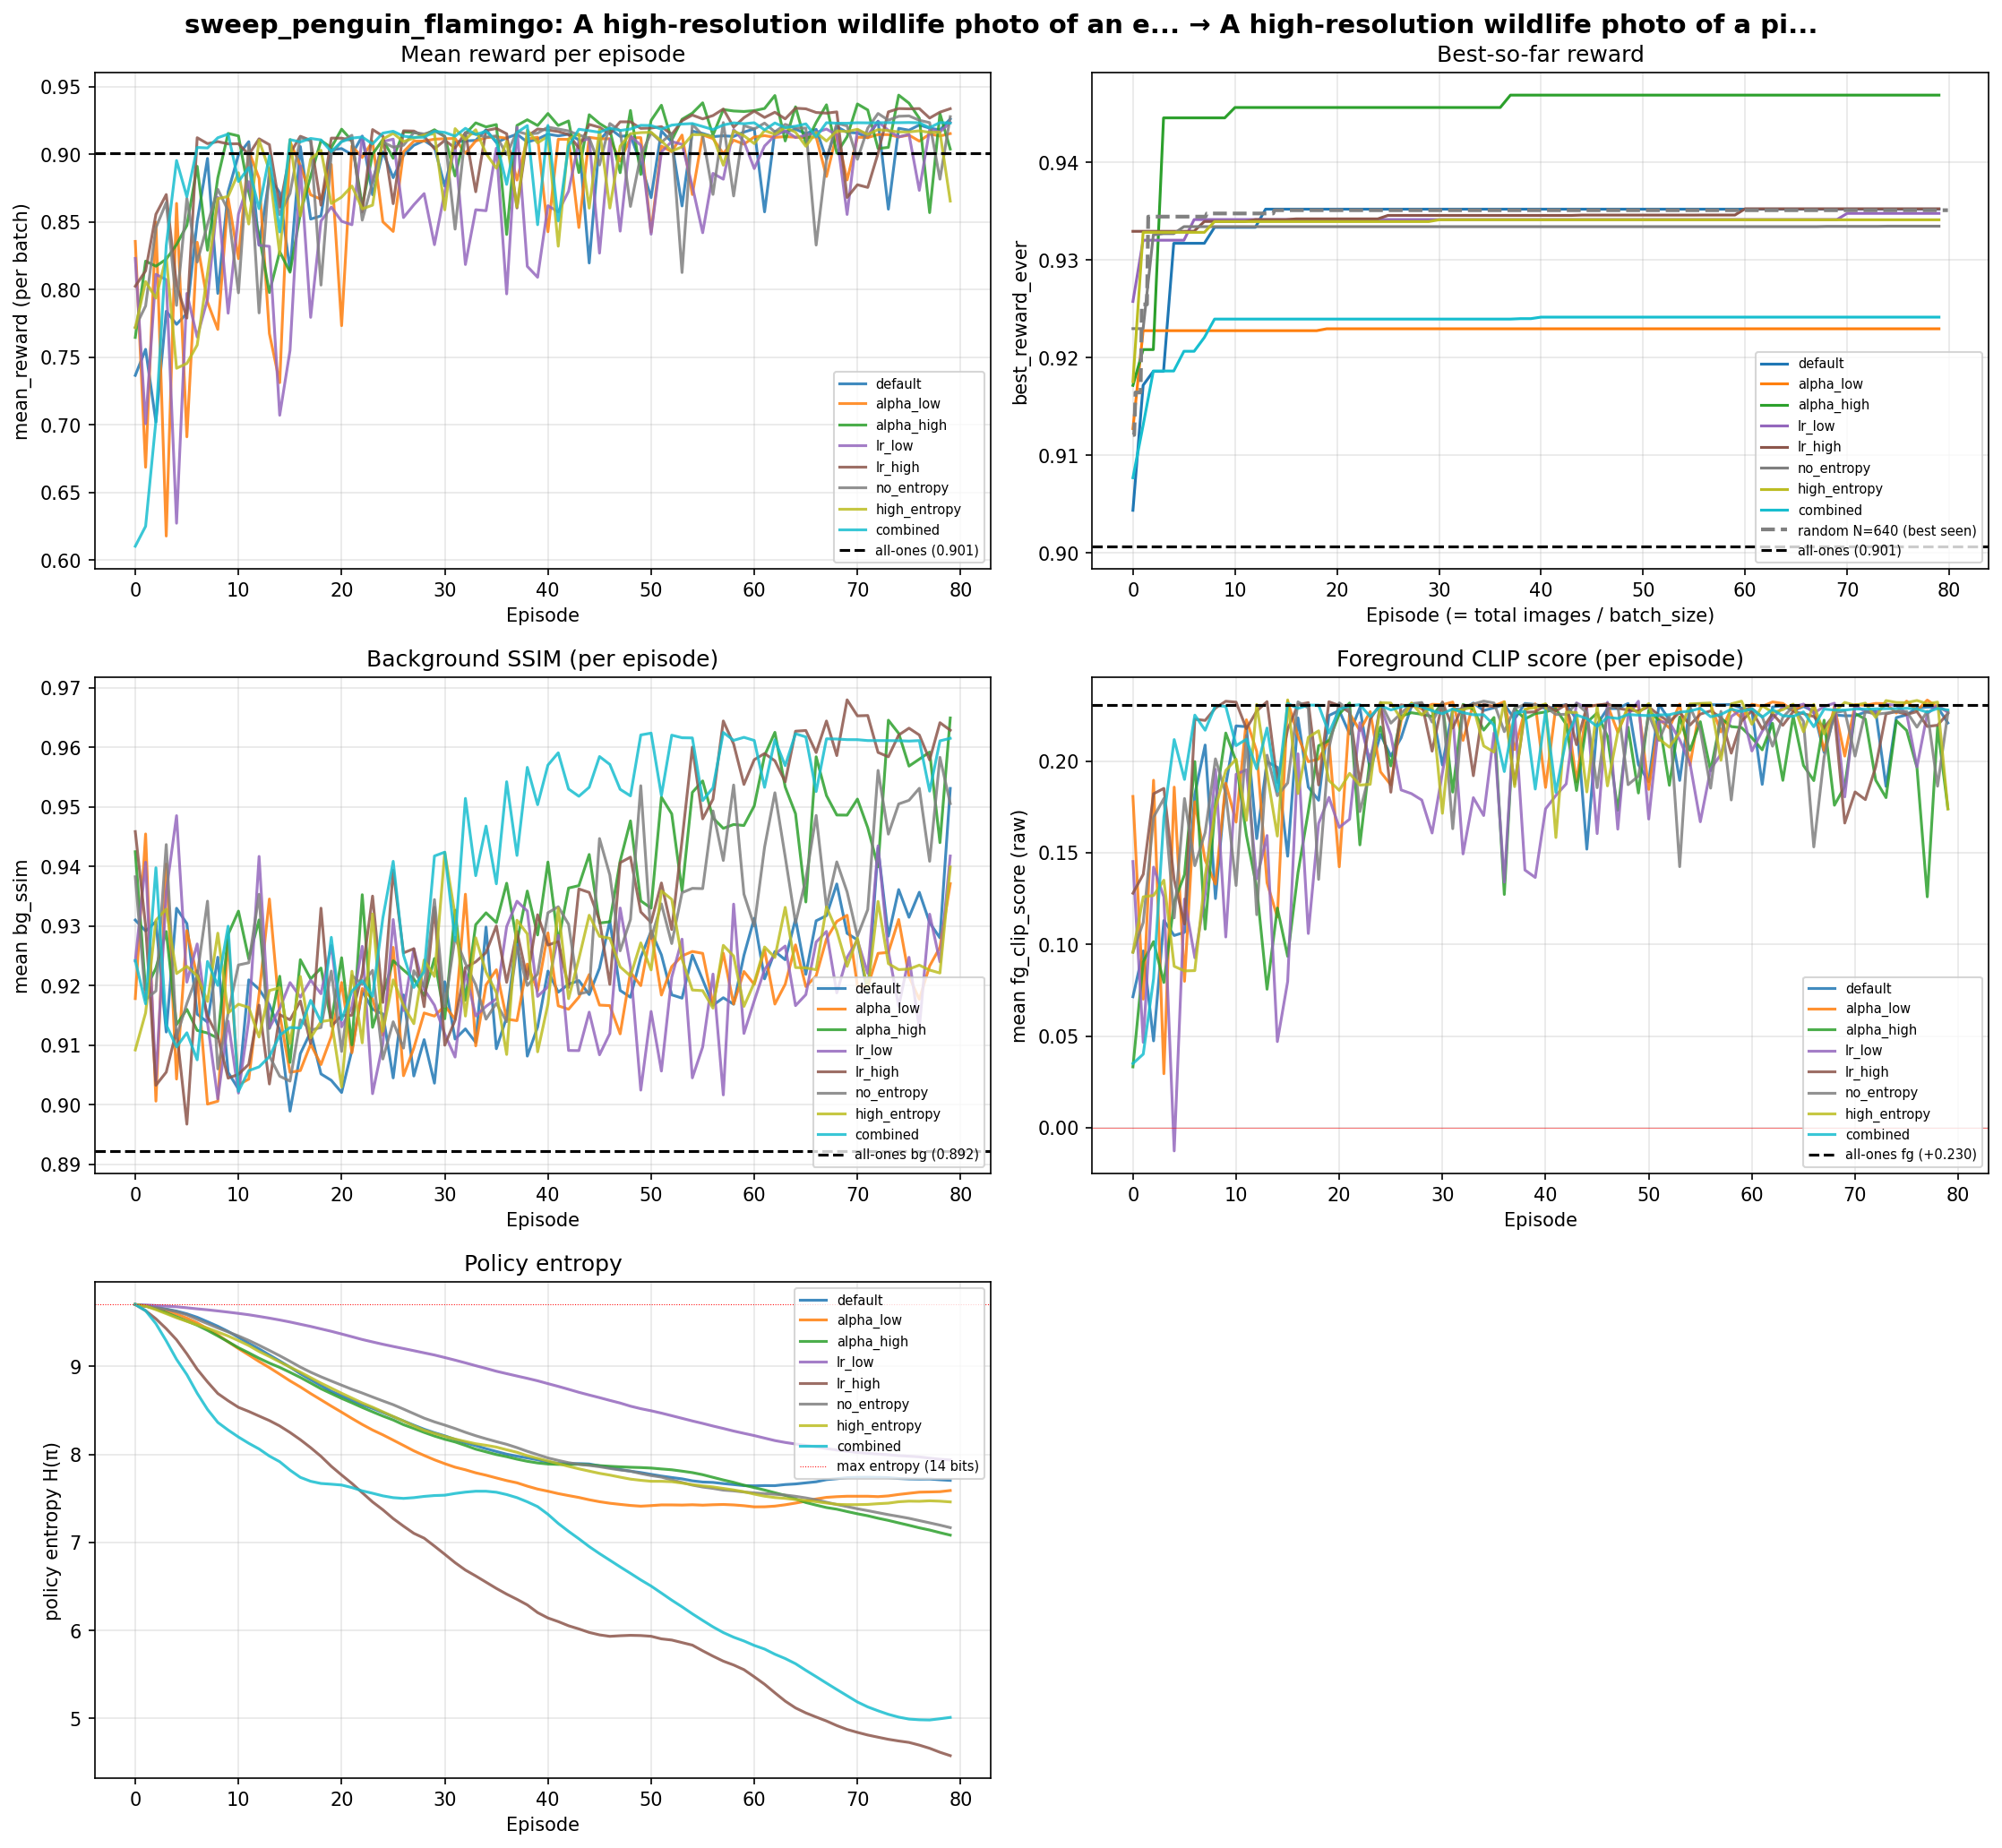
\includegraphics[width=\textwidth]{images/phase2/sweep_penguin_flamingo_curves.png}
    \caption{8-config sweep on \texttt{penguin\_flamingo}. All-ones reward $0.901$. Best config \texttt{alpha\_high} reaches $0.947$; random-640 best $0.935$.}
    \label{fig::sweep_penguin}
\end{figure}

The $\alpha=0.7$ (``alpha\_high'') config wins or ties on 5 of 6 sweep edits; it loses only on \texttt{bgrich\_candle\_crystal} where the scene's natural bg\_ssim is low and the policy benefits from pushing foreground harder. We freeze $\alpha=0.7$ for the 15-edit suite of Section~\ref{sec:experiments_new_bgrich}. Variations in learning rate and entropy coefficient within the swept range ($\eta\in[10^{-3}, 5\cdot 10^{-2}]$, $\beta\in[0, 0.1]$) move the final reward by at most $0.02$, so the method tolerates these hyperparameters.

\section{Random search at matched budget}
\label{sec:experiments_random}

Does the policy learn, or does matched-budget random do the same work? For each of the 6 sweep edits we sampled 640 uniform-random Bernoulli masks ($p=0.5$), the same image budget as an 80-episode REINFORCE run. Figure~\ref{fig::reward_histograms14} plots the reward distribution of those 640 samples; the red vertical line marks the REINFORCE final best.

\begin{figure}[H]
    \centering
    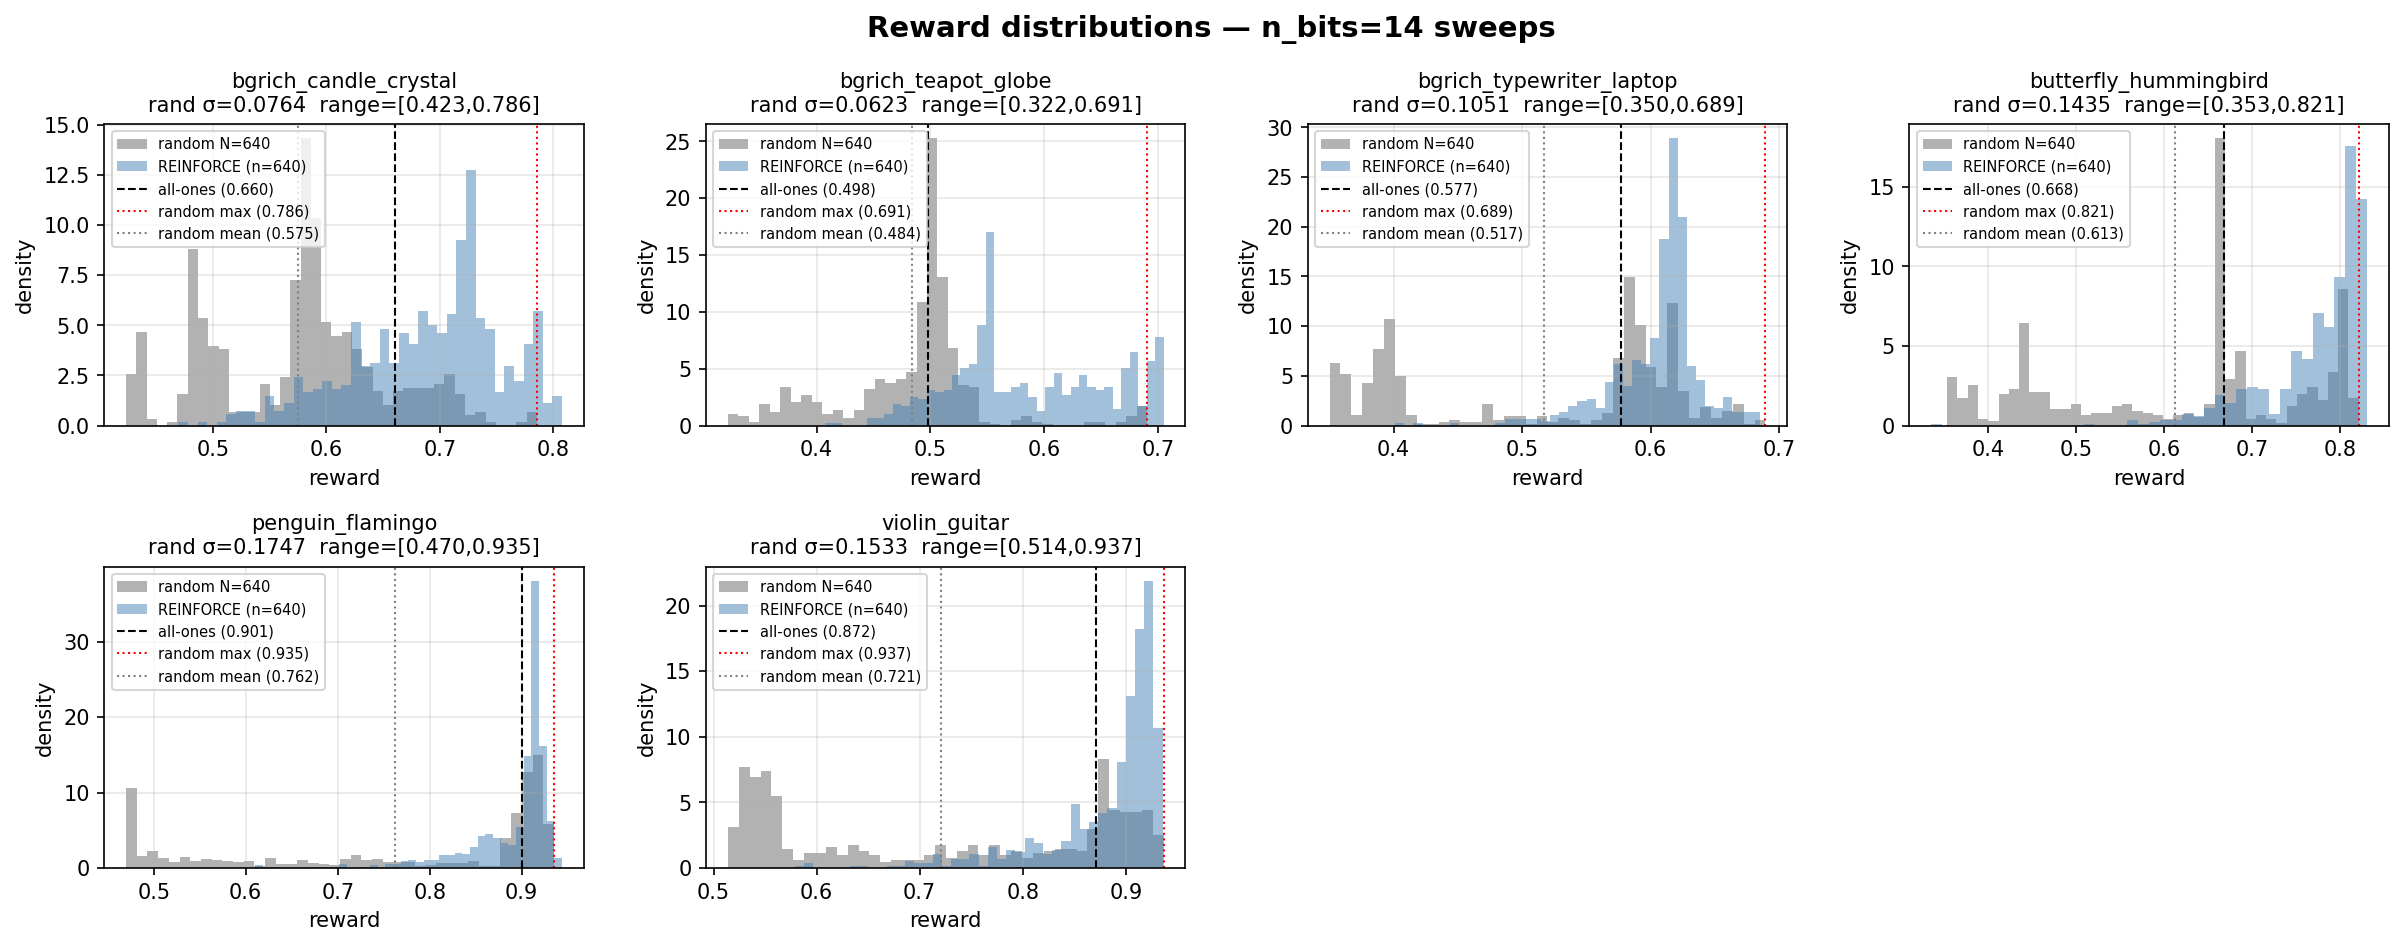
\includegraphics[width=\textwidth]{images/phase2/reward_histograms_nbits14.png}
    \caption{Reward histograms of 640 uniform-random masks per edit ($N=14$). REINFORCE's best (red line) sits in the right tail of the random distribution, narrowly above the random max (gap between $+0.6$ and $+2.3$ reward points per edit). The bigger win shows up on the \emph{mean} of the distribution: REINFORCE concentrates its batch on high-reward masks, while random spends most of its budget in the low-reward body.}
    \label{fig::reward_histograms14}
\end{figure}

On best-of-N the two methods sit close together: REINFORCE beats random-640 by $+0.6\%$ to $+2.3\%$ absolute reward. This best-of-N comparison understates the win for two reasons.

\paragraph{(a) REINFORCE shifts the whole distribution.} The policy's mean batch reward (Figure~\ref{fig::new_bgrich_curves}, top-left, thick black) plateaus near $0.73$; the random distribution's mean sits around $0.52$. On expected reward per generation, the gap is $+0.21$.

\paragraph{(b) REINFORCE returns a policy, not a sample.} Taking the greedy argmax of the learned Bernoulli produces a deterministic mask. The 640 generations compress into 14 logits. Random search cannot do that. Those logits can serve as supervision for a prompt-conditioned regressor, which turns per-edit search into single-shot inference (Chapter~\ref{ch:conclusion}).

\section{Qualitative comparison}

Figure~\ref{fig::visual_comparison} shows source, all-ones, and REINFORCE-top-1 outputs side by side for 21 background-rich edits. In every row the all-ones column damages some part of the scene (the Victorian study of globe$\to$orrery loses its warm amber light; the study of chess$\to$checkers loses the ornate book-lined background), while the REINFORCE-top-1 column keeps all of the background props and still commits the object swap.

\begin{figure}[H]
    \centering
    \begin{subfigure}[t]{0.32\textwidth}
        \centering
        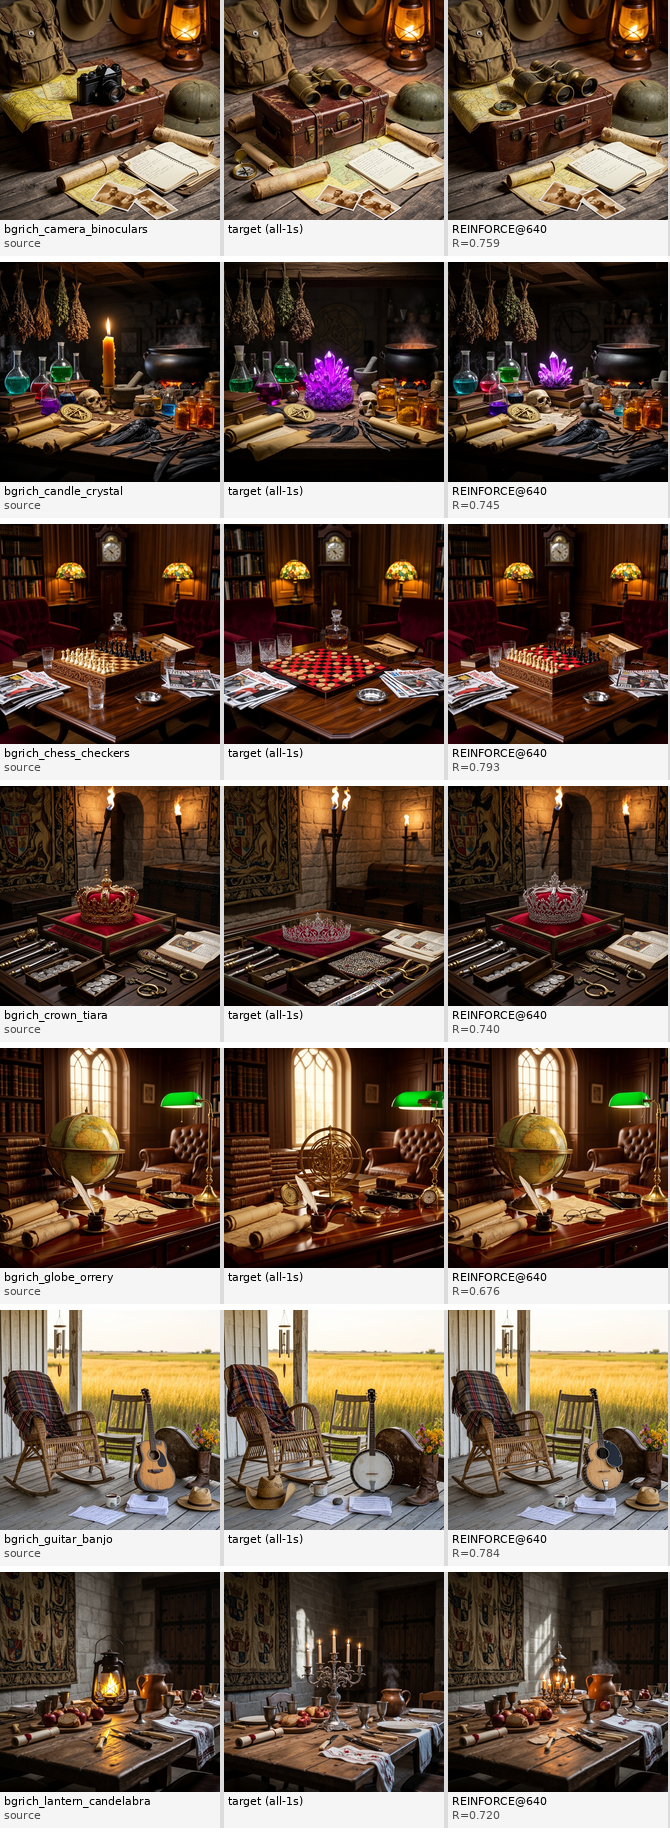
\includegraphics[width=\textwidth]{images/phase2/visual_comparison_part1.png}
        \caption{Tasks 1--7.}
    \end{subfigure}
    \hfill
    \begin{subfigure}[t]{0.32\textwidth}
        \centering
        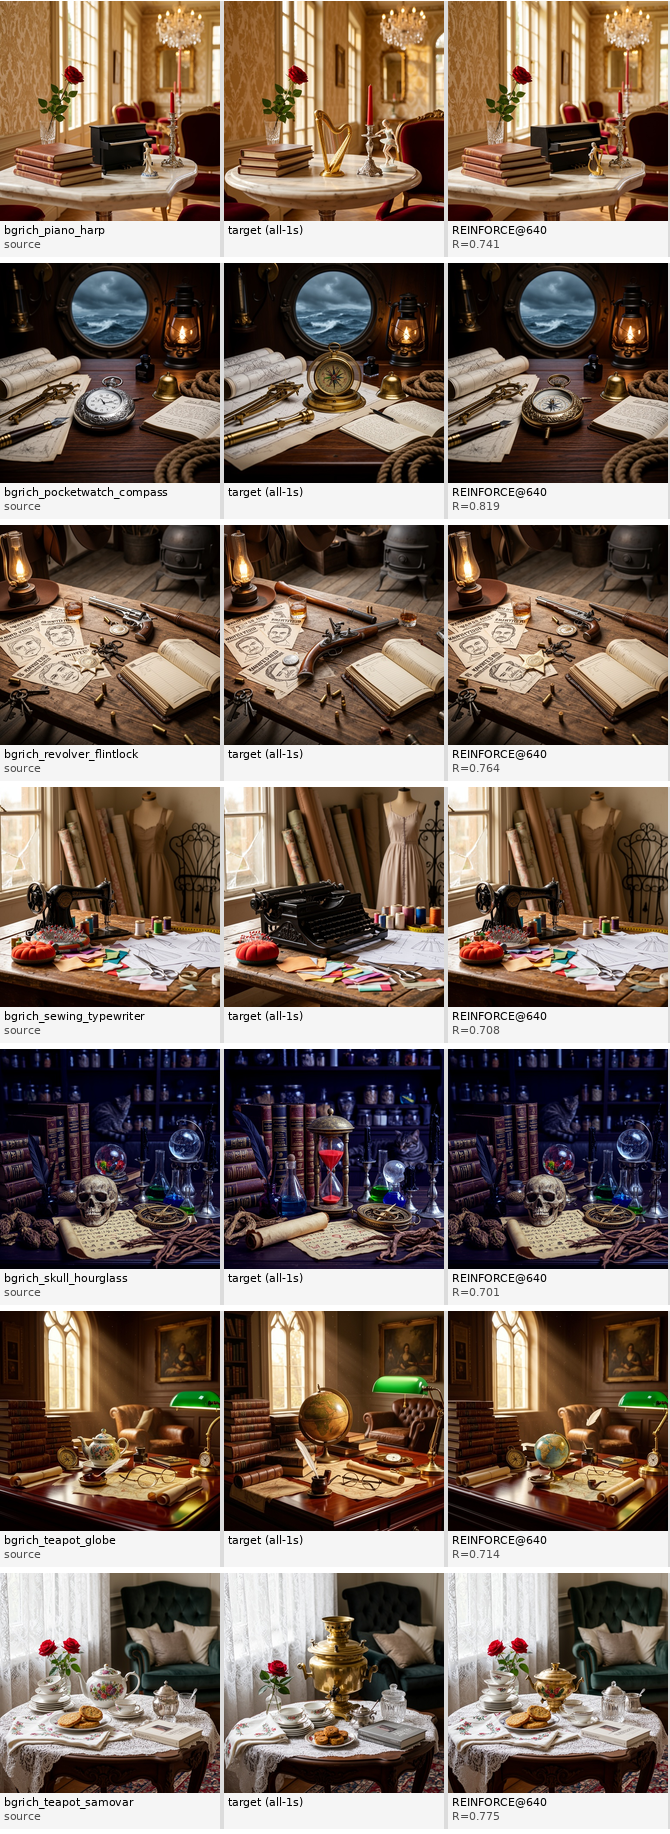
\includegraphics[width=\textwidth]{images/phase2/visual_comparison_part2.png}
        \caption{Tasks 8--14.}
    \end{subfigure}
    \hfill
    \begin{subfigure}[t]{0.32\textwidth}
        \centering
        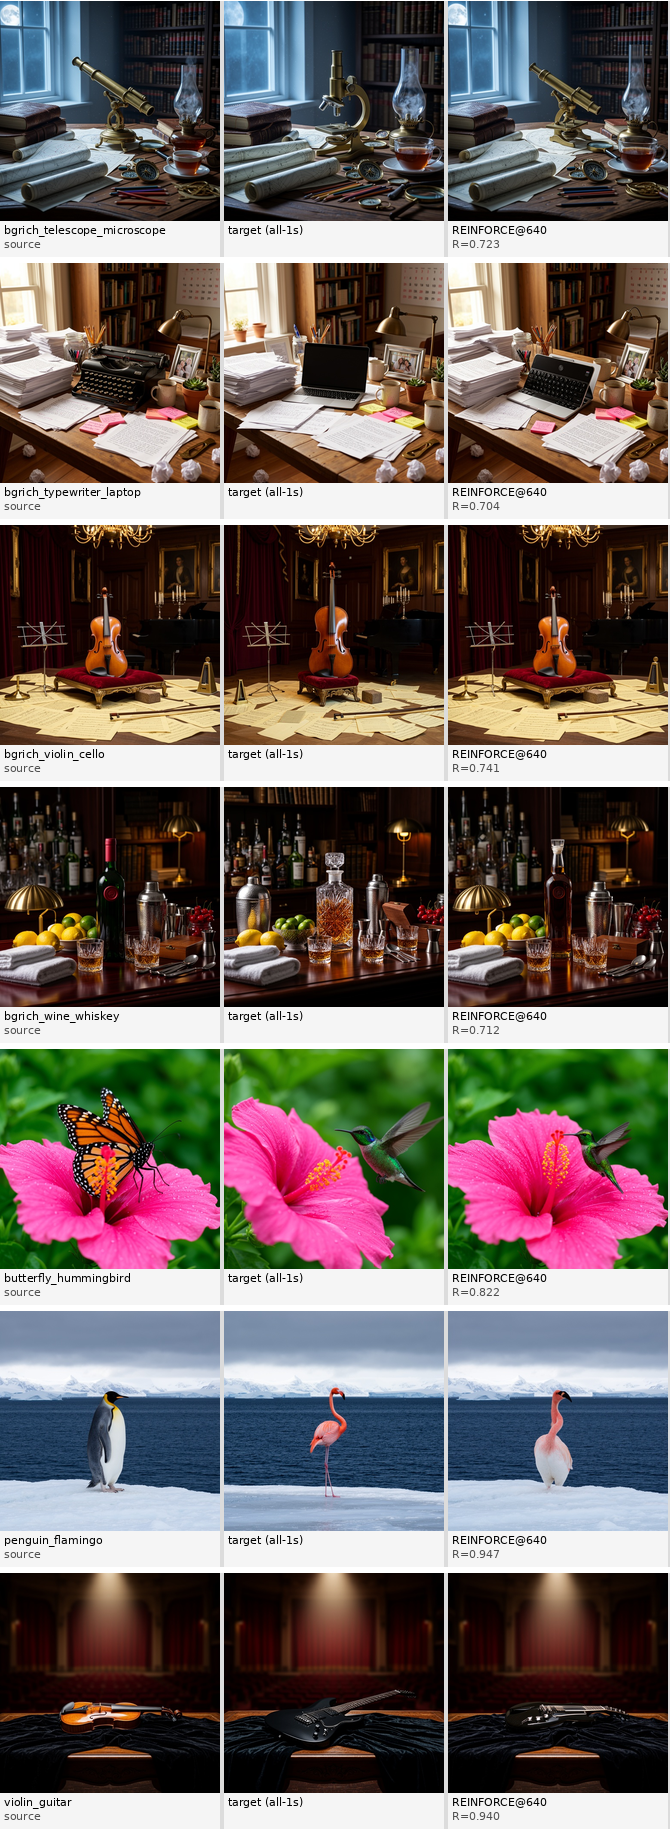
\includegraphics[width=\textwidth]{images/phase2/visual_comparison_part3.png}
        \caption{Tasks 15--21.}
    \end{subfigure}
    \caption{Qualitative comparison across 21 background-rich edits, split into three vertical strips for readability. In each strip, columns are source ($M=\mathbf{0}$), all-ones ($M=\mathbf{1}$), and REINFORCE top-1 ($\hat{M}$ after training). All-ones keeps the object but damages the scene; REINFORCE-top-1 keeps both.}
    \label{fig::visual_comparison}
\end{figure}
